




In \secref{prior_perturbations} we considered a multiplicative perturbations
of the form \eqref{phi_perturbation} with the $\norminf{\cdot}$ norm.  In
this section we consider other norms, illustrating that other choices
have problems with KL divergence.

First, we recall what we hope to get from our linear approximation.  We wish to
approximation $\etaopt(\phi)$ using the linear approximation $\etalin(\phi)$
evaluated at $\phiz$, hoping that the error $\norm{\etaopt(\phi) -
\etalin(\phi)}_2$ is small whenever the $\norm{\phi}$ is small (for some choice
of $\norm{\cdot}$).  A bare minimum for such a local approximation to work is
for $\phi \mapsto \etaopt(\phi)$ to be continuous, so that, for any
$\phi$,
%
\begin{align*}
%
\lim_{t \rightarrow 0} \norm{\etaopt(t \phi) - \etaopt}_2 = 0.
%
\end{align*}
%
By this reasoning, however, $\etaopt$ itself is a ``good'' approximation to
$\etaopt(\phi)$ when $\norm{\phi}$ is small---when $\phi$ is small, by
continuity we can simply say that nothing has changed and be reasonably correct.
From our linear approximation, we expect another order of accuracy, namely that
%
\begin{align*}
%
\lim_{t \rightarrow 0} \frac{\norm{\etaopt(t \phi) - \etalin(t\phi)}_2}{t} = 0.
%
\end{align*}

The preceding display is enough if we have a fixed $\phi$ in mind.  However, if
we want to search over a larger set of candidate $\phi$, we want the derivative
to provide a {\em uniformly good approximation} to $\etaopt(\phi)$ amonst some
set of $\phi$, say, all bounded $\phi: \norm{\phi} \le 1$.  One way of
formalizing the notion of ``uniformaly good approximation'' follows.

%%%%%%%%%%%%%%%%%%%%%%%%%%%%%%%%%%%%%%%%%%%%%%%%%%%%%%%%%%%%%%%%%%%%%%%%%%%
%%%%%%%%%%%%%%%%%%%%%%%%%%%%%%%%%%%%%%%%%%%%%%%%%%%%%%%%%%%%%%%%%%%%%%%%%%%
\begin{defn}\deflabel{diffable_classes}
    (\citep[Definition 4.5]{zeidler:2013:functional})
%
Let $B_1$ and $B_2$ denote Banach spaces, and let $\ball_1 \subseteq B_1$ define
an open neighborhood of $\phi_0 \in B_1$.  Fix a function $f: \ball_1
\mapsto B_2$.

The function $f$ is {\em directionally differentiable} (also known as a Gateaux
differentiable) if there exists a bounded linear functional $f^{\mathrm{lin}}:
B_1 \mapsto B_2$ such that the following condition holds for any
$\phi$ with $\norm{\phi - \phi_0} < \infty$:
%
\begin{align*}
%
%\textrm{For any }\phi\textrm{ with }\norm{\phi - \phi_0} < \infty\textrm{, }
\lim_{t \rightarrow 0}
    \frac{f(\phi) - f(\phi_0) -
          f^{\mathrm{lin}}(t (\phi - \phi_0) )
         }{t} \rightarrow 0.
%
\end{align*}
%

Similarly, the function $f$ is {\em boundedly differentiable} (also known as
Fr{\'echet} differentiable) at $\phi_0$ if we can take the limit uniformly in
$\phi$:
%
\begin{align*}
%
\lim_{t \rightarrow 0}
    \sup_{\phi: \norm{\phi - \phi_0} = 1}
    \frac{f(\phi) - f(\phi_0) -
          f^{\mathrm{lin}}(t (\phi - \phi_0))
         }{t} \rightarrow 0.
%
\end{align*}
%
\end{defn}
%%%%%%%%%%%%%%%%%%%%%%%%%%%%%%%%%%%%%%%%%%%%%%%%%%%%%%%%%%%%%%%%%%%%%%%%%%%

Note that we used the same notation $f^{\mathrm{lin}}$ for both derivatives in
\defref{diffable_classes}.  In fact, if a function is compactly differentiable
then the two derivatives must coincide \citep[Proposition
4.8]{zeidler:2013:functional}, which justifies our presumptuous notation.

% The difference between bounded and directional differentiability is whether the
% linear approximation holds uniformly in $\phi$.

It is possible for functions to be directionally but not boundedly
differentiable even in $\mathbb{R}^2$, as the following example demonstrates.

%%%%%%%%%%%%%%%%%%%%%%%%%%%%%%%%%%%%%%%%%%%%%%%%%%%%%%%%%%%%%%%%%%%%%%%%%
%%%%%%%%%%%%%%%%%%%%%%%%%%%%%%%%%%%%%%%%%%%%%%%%%%%%%%%%%%%%%%%%%%%%%%%%%
\begin{ex}\exlabel{r2_pathological}
%
Consider $(x_1, x_2) \in \mathbb{R}^2$ and the polar coordinates $r :=
\sqrt{x_1^2 + x_2^2}$ and $\theta := \arctan(x_2 / x_1)$.  Let $\{\pi k: k \in
\mathbb{Z} \}$ denote integer multiples of $\pi$.  Define
%
% \begin{align*}
% %
% f(r, \theta) := \begin{cases}
% \frac{\left(\frac{r}{| \sin \theta |}\right)^2}
%      {1 + \left(\frac{r}{| \sin \theta |}\right)^2}
%     & \textrm{when } \theta \notin \{\pi k: k \in \mathbb{Z}\}
%     \textrm{ and } r > 0 \\
% 0. & \textrm{when } \theta \in \{\pi k: k \in \mathbb{Z}
%     \} \textrm{ or }r = 0
% %
% \end{cases}
\begin{align*}
%
f(r, \theta) := \begin{cases}
    \left(\frac{r}{| \sin \theta |}\right)^2
        & \textrm{when } \theta \notin \{\pi k: k \in \mathbb{Z}\}
        \textrm{ and } r > 0 \\
    0. & \textrm{when } \theta \in \{\pi k: k \in \mathbb{Z}
        \} \textrm{ or }r = 0
%
\end{cases}
%
\end{align*}
%
%%%%%%%%%%%%%%%%%%%%%%%%%%%%%%%%%%%%%%%%%%%%%%%%%%%%%%%%%%%%%%%%%%%%%%%%%
%%%%%%%%%%%%%%%%%%%%%%%%%%%%%%%%%%%%%%%%%%%%%%%%%%%%%%%%%%%%%%%%%%%%%%%%%
\begin{figure}[h!]

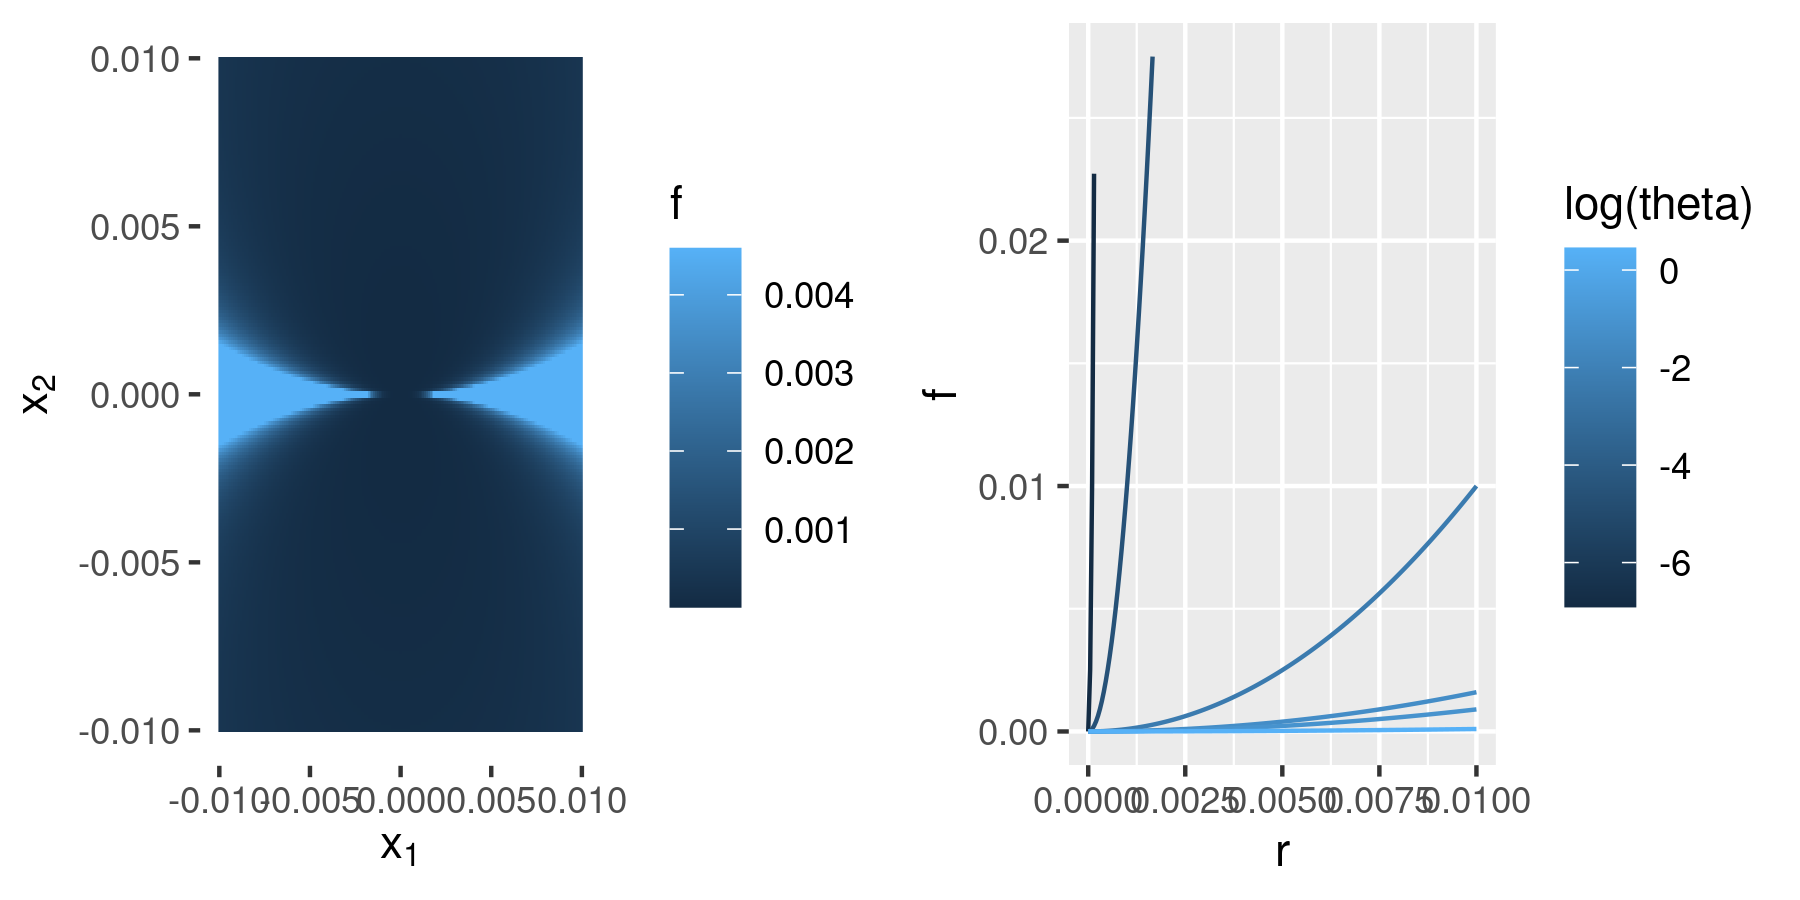
\includegraphics[width=0.980\linewidth,height=0.490\linewidth]{static_images/pathological_r2_example.png}
\caption{A plot of $f(x_1, x_2)$ from \exref{r2_pathological}.}
\figlabel{r2_pathological}
\centering
\end{figure}
%%%%%%%%%%%%%%%%%%%%%%%%%%%%%%%%%%%%%%%%%%%%%%%%%%%%%%%%%%%%%%%%%%%%%%%%%
%
\Figref{r2_pathological} contains a plot of $f(r, \theta)$, both over
$\mathbb{R}^2$ and along paths for particular choices of $\theta$.

Then $f$ has a directional derivative in every direction, but is not Fr{\'e}chet
differentiable.  By ordinary calculus, for any $\theta$, $\fracat{\partial f(r,
\theta)}{\partial r}{r=0} = 0$, so the directional derivatives all exist and are
identically $0$.  However, for any $r$, there exists a $\theta(r)$ such that $r /
|\sin(\theta(r))| = 1$.  For such a choice of $\theta(r)$, the error in the
linear approximation is $f(r, \theta(r)) - 0 = 1/2$, which does not go to zero
as $r \rightarrow 0$.

\end{ex}
%%%%%%%%%%%%%%%%%%%%%%%%%%%%%%%%%%%%%%%%%%%%%%%%%%%%%%%%%%%%%%%%%%%%%%%%%

Note that the second derivative in a particular direction is given by
$\fracat{\partial^2 f(r, \theta)}{\partial r^2}{r=0} = \frac{1}{2 |\sin
\theta|}$, which can be made arbitrarily large by taking $\theta$ close to $0$
or to $\pi$.  We could modify $f(r, \theta)$ to be Fr{\'e}chet differentiable
by smoothly ``capping'' $1 / |\sin \theta|$ at some arbitrarily large value.
However, the ability to meaningfully extrapolate $f(r, \theta)$ in the direction
of a very large but finite second derivative will still be extremely limited. In
this sense, Fr{\'e}chet differentiability is a weak necessary but not sufficient
requirement if we are interested in extrapolating using linear approximations.



%%%%%%%%%%%%%%%%%%%%%%%%%%%%%%%%%%%%%%%%%%%%%%%%%%%%%%%%%%%%%%%%%%%%%%%%%
%%%%%%%%%%%%%%%%%%%%%%%%%%%%%%%%%%%%%%%%%%%%%%%%%%%%%%%%%%%%%%%%%%%%%%%%%
\begin{ex}\exlabel{r2_pathological_v2}
%
In the context of \exref{r2_pathological}, fix some $0 < M < \infty$,
and define
%
\begin{align*}
%
\tilde{f}(r, \theta) := \begin{cases}
    f(r, \theta) & \textrm{when }\frac{1}{\abs{\sin(\theta)}} \le M \\
    0. & \textrm{when }\frac{1}{\abs{\sin(\theta)}} > M.
%
\end{cases}
%
\end{align*}
%
Then $\tilde{f}$ is continuous and Fr{\'e}chet differentiable at $r=0$. In this
case, for any $r$, $\sup_{\theta} r / |\sin(\theta(r))| = r / M$, so  both
$\lim_{r \rightarrow 0} \tilde{f}(r, \theta) \le \lim_{r \rightarrow 0} r^2 /
M^2 = 0$ and $\lim_{r \rightarrow 0} \tilde{f}(r, \theta) / r \le \lim_{r
\rightarrow 0}  r / M^2 = 0$.  (Note that $\tilde{f}$ is continuous only
at $r=0$, not on a ball centered at $0$.)

Despite being Fr{\'e}chet differentiable, the linear approximation may not
extrapolate well to any finite $r$.  In the direction $\theta = \sin^{-1}(1 /
M)$, the error of the linear extrapolation to any $r_0$ is still $\tilde{f}(r,
\theta) - 0 = M r_0^2$. Since Fr{\'e}chet differentiability requires only $M <
\infty$, the extraplation error can be arbitrarily large, even for Fr{\'e}chet
differentiable functions.

\end{ex}
%%%%%%%%%%%%%%%%%%%%%%%%%%%%%%%%%%%%%%%%%%%%%%%%%%%%%%%%%%%%%%%%%%%%%%%%%


\Exref{r2_pathological} is neither Fr{\'e}chet differentiable nor continuous,
whereas \exref{r2_pathological} is both Fr{\'e}chet differentiable and
continuous.  In general, however, Fr{\'e}chet differentiability is stronger than
continuity, in the sense that Fr{\'e}chet differentiability implies continuity,
but continuity does not imply Fr{\'e}chet differentiability \citep[Proposition
4.8 (d)]{zeidler:2013:functional}.  See also \citet[Example
1.9]{averbukh:1967:theory} for a simple example of a function on $\mathbb{R}^2$
that is continuous and directionally differentiable but not Fr{\'e}chet
differentiable.

The sort of pathology exhibited by \exref{r2_pathological, r2_pathological_v2}
requires some care to construct in $\mathbb{R}^2$, but requires some care to
avoid in infinite-dimensional spaces.  We now give an illustrative example in
the $\lp{p}$ spaces; since the result will be important for VB prior
sensitivity, we will state is as a lemma rather than merely an example.

We can define the family of nonlinear perturbations similar to
\citep{gustafson:1996:local}.


%%%%%%%%%%%%%%%%%%%%
%%%%%%%%%%%%%%%%%%%%
%%%%%%%%%%%%%%%%%%%%
%%%%%%%%%%%%%%%%%%%%
%%%%%%%%%%%%%%%%%%%%
%%%%%%%%%%%%%%%%%%%%


Of course, if we relax the constraint that $\phi(\nu) \ge 0$, then we cannot
guarantee that $\pstick(\nu \vert \phi) \ge 0$ in an open ball around $\phiz$.

It will be notationaly convenient in our discussion to treat the map $x \mapsto
\log(x)$ as simply discontinuous at $x = 0$, rather than undefined (or
complex-valued). Define the ``trimmed log'' function as

%%%%%%%%%%%%%%%%%%%%%%%%%%%%%%%%%%%%%%%%%%%%%%%%%%%%%%%%%%%%%%%%%%%%%%%%%
%%%%%%%%%%%%%%%%%%%%%%%%%%%%%%%%%%%%%%%%%%%%%%%%%%%%%%%%%%%%%%%%%%%%%%%%%
\begin{defn}
%
\begin{align*}
%
\logtrim(x) :=
\begin{cases}
    \log x  &\textrm{when }x > 0 \\
    0       &\textrm{when }x \le 0.
\end{cases}
%
\end{align*}
%
% In order for the directional derivative to exist in the direction of
% functions unbounded below, the value must be \log(1) = zero when undefined
%
% Otherwise, the when $x \le 0$ is simply a placeholder; for our purposes, it would
% ideally be some abstract number that is distant from all real numbers but zero
% distance to itself.  (Neither $0$ nor $\infty$ quite fit the bill.) Mostly we
% will require that $\logtrim(x)$ is discontinuous in a neighborhood of $0$.
%
\end{defn}
%%%%%%%%%%%%%%%%%%%%%%%%%%%%%%%%%%%%%%%%%%%%%%%%%%%%%%%%%%%%%%%%%%%%%%%%%

Observe, that, for $1 \le p < \infty$, we take the log perturbation given by
\defref{prior_nl_pert} is
%
\begin{align*}
%
\logtrim \p(\theta \vert \phi) ={}&
    \log \pbase(\theta) +
        \logtrim\left(1 + \frac{\phi(\theta)}{\pbase(\theta)^{1/p}} \right).
%
\end{align*}
%


We can now state our main results.


\begin{thm}
%
Fix $1 \le p < \infty$ and define a prior perturbation as in
\defref{prior_nl_pert}.
Assume that the variational approximations $\q(\nu \vert \etanuk)$ to the
stick-breaking posteriors satisfy \assuref{dist_fun_nice} with $\eta_0 =
\etaopt$, with $\psi(\zeta, \t) = 1$, and with $\psi(\zeta, \t) = \log\left(1 + \frac{\phi(\nu)}{\pbase(\nu)^{1/p}} \right)$, for all $\k$.

%
\end{thm}
